\documentclass[a4paper, 12pt]{report}

%====================== PACKAGES ======================

\usepackage[french]{babel}
\usepackage[utf8x]{inputenc}
%pour gérer les positionnement d'images
\usepackage{float}
\usepackage{amsmath}
\usepackage{graphicx}
\usepackage[colorinlistoftodos]{todonotes}
\usepackage{url}
%pour les informations sur un document compilé en PDF et les liens externes / internes
\usepackage{hyperref}
%pour la mise en page des tableaux
\usepackage{array}
\usepackage{tabularx}
%pour utiliser \floatbarrier
%\usepackage{placeins}
%\usepackage{floatrow}
%espacement entre les lignes
\usepackage{setspace}
%modifier la mise en page de l'abstract
\usepackage{abstract}
%police et mise en page (marges) du document
\usepackage[T1]{fontenc}
\usepackage[top=2cm, bottom=2cm, left=2cm, right=2cm]{geometry}
%Pour les galerie d'images
\usepackage{subfig}
\usepackage[rightcaption]{sidecap}
\graphicspath{ {images/} }

%====================== INFORMATION ET REGLES ======================

%rajouter les numérotation pour les \paragraphe et \subparagraphe
\setcounter{secnumdepth}{4}
\setcounter{tocdepth}{4}

\hypersetup{							% Information sur le document
pdfauthor = {Sugdenaz EKICI,
			Yahia KHERZA,
			Olivier MARAVAL,
    		Valentin VIRET-JACQUOT},			% Auteurs
pdftitle = {1_Analyse},			% Titre du document
pdfsubject = {Mémoire de Projet},		% Sujet
pdfkeywords = {Tag1, Tag2, Tag3, ...},	% Mots-clefs
pdfstartview={FitH}}					% ajuste la page à la largueur de l'écran
%pdfcreator = {MikTeX},% Logiciel qui a crée le document
%pdfproducer = {}} % Société avec produit le logiciel

%======================== DEBUT DU DOCUMENT ========================

\begin{document}

\addtocontents{toc}{\protect\thispagestyle{empty}}

%régler l'espacement entre les lignes
\newcommand{\HRule}{\rule{\linewidth}{0.5mm}}

%page de garde
\begin{titlepage}
\begin{center}

% Upper part of the page. The '~' is needed because only works if a paragraph has started.

\includegraphics[width=0.5\textwidth]{./images/InfoLogoQuadriH.png}~\\[1cm]

\textsc{\LARGE SAE 1.04 - BUT INFORMATIQUE - GROUPE 1}\\[1.5cm]

\textsc{\Large }\\[0.5cm]

% Title
\HRule \\[0.4cm]

{\huge \bfseries Analyse des besoins de l'entreprise\\
 LOCECO\\[0.4cm] }

\HRule \\[1.5cm]

% Author and supervisor
\begin{minipage}{0.4\textwidth}
\begin{flushleft} \large
\emph{Auteur:}\\
Sugdenaz \textsc{Ekici}(\textit{A1})\\
Yahia \textsc{Kherza}(\textit{A1})\\
Olivier \textsc{Maraval}(\textit{A1})\\
Valentin \textsc{Viret-Jacquot}(\textit{A1})
\end{flushleft}
\end{minipage}
\begin{minipage}{0.4\textwidth}
\begin{flushright} \large
\emph{Client:} \\
Karine \textsc{Deschinkel}\\
\emph{Référent:} \\
Olivier \textsc{Maraval}
\end{flushright}
\end{minipage}

\vfill

% Bottom of the page
{\large \today}

\end{center}
\end{titlepage}

%page blanche
\newpage
~
\thispagestyle{empty}


\tableofcontents
\thispagestyle{empty}

\listoffigures
\thispagestyle{empty}

\newpage

%espacement entre les lignes d'un tableau
\renewcommand{\arraystretch}{1.5}

%====================== INCLUSION DES PARTIES ======================

~
\thispagestyle{empty}


\newpage

\chapter{Analyse de l'existant}

\section{Les écoquartiers}

\subsection{Présentation du concept d'écoquartier}

Un écoquartier est un quartier urbain conçu de manière à être respectueux de l'environnement et à promouvoir le développement durable. Il intègre des principes tels que la gestion efficace des ressources, la réduction des émissions de carbone, la promotion de la mobilité douce et l'utilisation d'énergies renouvelables.\\

Le fonctionnement d'un écoquartier repose sur plusieurs principes clés :
\begin{itemize}
\item \textbf{La gestion efficace des ressources :} un écoquartier vise à minimiser la consommation d'eau et d'énergie, ainsi que la production de déchets. Cela peut se faire en utilisant des technologies d'énergie renouvelable, en encourageant la réutilisation et le recyclage des matériaux, ou encore en favorisant les modes de transport doux comme le vélo ou les transports en commun.
\item \textbf{La conception urbaine durable :} un écoquartier est conçu pour encourager la cohésion sociale, en offrant des espaces verts et des lieux de rencontre pour les résidents. Il doit également être accessible à tous, notamment aux personnes à mobilité réduite.
\item \textbf{La participation des résidents :} les habitants de l'écoquartier sont encouragés à participer activement à la gestion du quartier, en prenant part aux décisions concernant l'aménagement et l'utilisation des espaces communs.
\item \textbf{La promotion de l'économie locale :} un écoquartier peut encourager l'installation d'entreprises locales et durables, favorisant ainsi l'emploi et l'économie locale.
\end{itemize}


\subsection{Exemple d'écoquartier}

Le quartier Vauban à Fribourg-en-Brisgau, en Allemagne est un exemple d'écoquartier. Ce dernier est conçu de manière à encourager la marche à pied et le vélo, avec des rues piétonnes et des pistes cyclables bien développées. 

Il utilise également des technologies d'énergie renouvelable, telles que l'énergie solaire, pour alimenter les bâtiments. De plus, le quartier favorise la cohésion sociale en encourageant la participation des résidents à la gestion du quartier et en offrant des espaces verts et des jardins communautaires.

\begin{figure}[!h]
\begin{center}
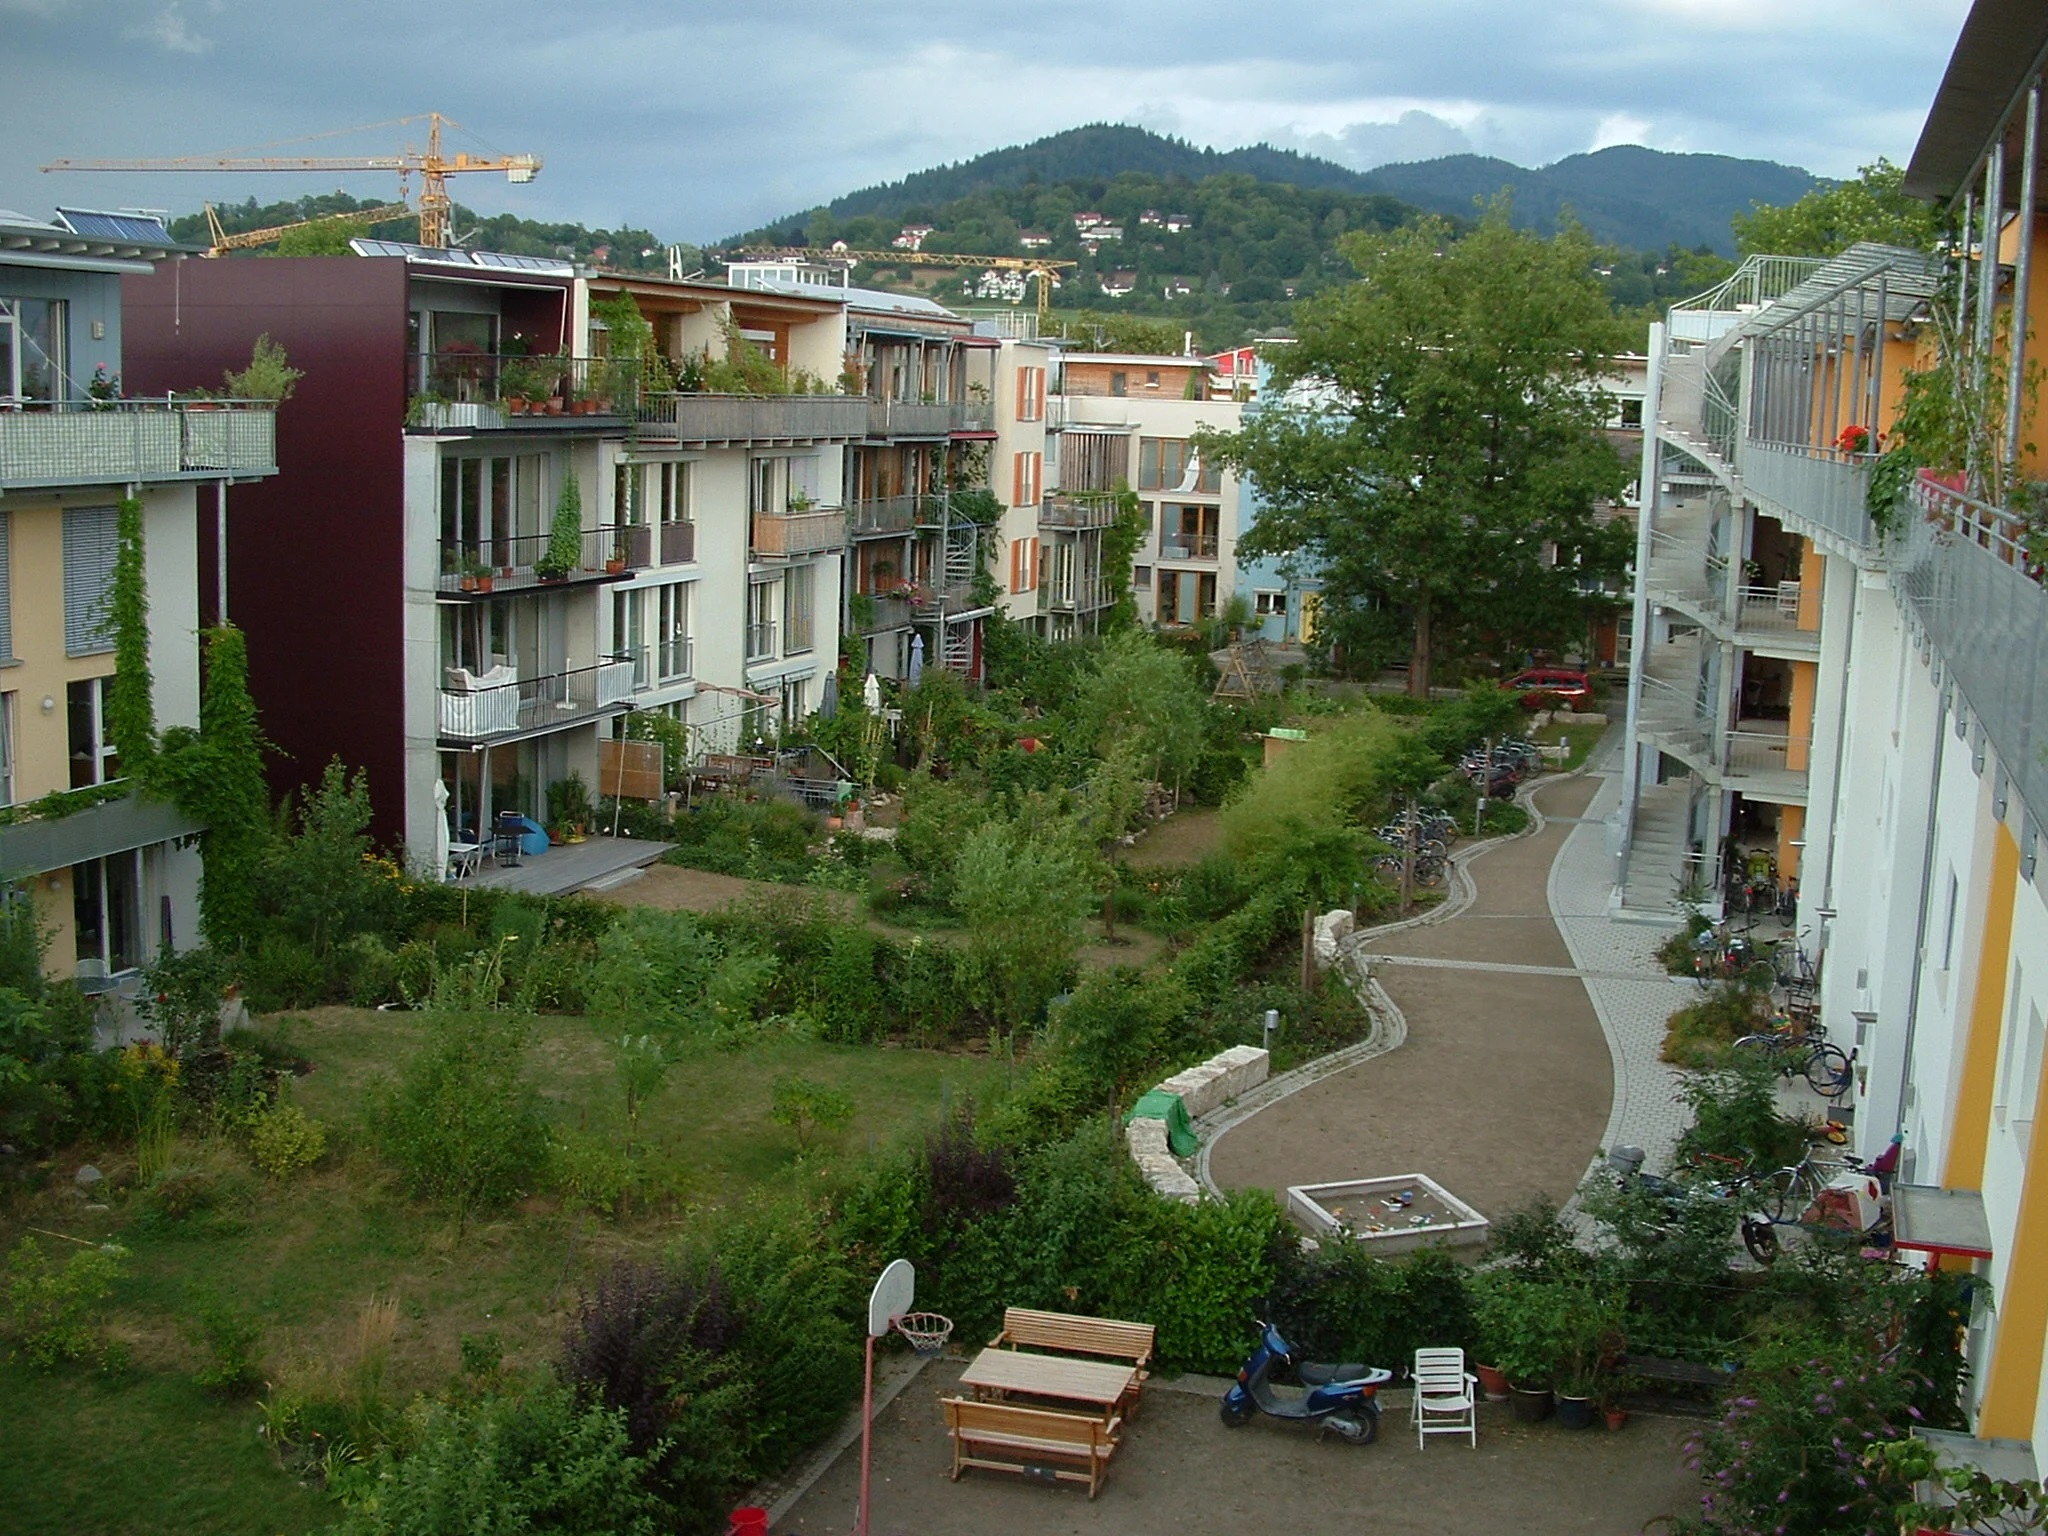
\includegraphics[width=15cm]{vauban-10029.jpg}
\end{center}
\caption{Le quartier Vauban à Fribourg-en-Brisgau}
\end{figure}

\newpage

\section{L'entreprise et l'écoquartier}

\subsection{Présentation de LOCECO}

LOCECO est une entreprise engagée dans la gestion et la location d’appartements au sein d’un quartier écologique. Ils gèrent leurs appartements de manière responsable en minimisant la consommation d’énergie.\\

LOCECO souhaite promouvoir une démarche de consommation durable auprès de ces locataires. Pour encourager les résidents à trier leurs déchets et à recycler autant que possible, de multiples poubelles de tri sélectif sont disponibles dans les parties communes et des campagnes de sensibilisation pour expliquer aux résidents l'importance de cette pratique sont régulièrement organisées.

\subsection{Présentation d'une entreprise similaire : La SERS}

La SERS est une entreprise qui se spécialise dans l'aménagement de l'espace urbain et la construction d'écoquartiers dans le Grand Est de la France.\\

Elle vise à intégrer les principes du développement durable dans ses projets, notamment en ce qui concerne la mobilité, la gestion des déchets, l'empreinte environnementale et la mixité sociale. Par ailleurs, elle a défini un certains nombres de critères qui permet d’offrir un cadre de vie sain et sûr à ses habitants.\\

Un exemple concret de la part de cette entreprise est l'écoquartier "Les Prairies du Canal"

Le programme d’aménagement de ce quartier conçu par la SERS vise à offrir une cohérence environnementale avec une présence de la nature dans l’architecture. La hauteur est privilégiée pour libérer plus de 80\% d’emprise au sol. Ce site de 14 ha et de 1 300 logements à terme offre des qualités paysagères dont la principale est sans nul doute la présence du canal.

\begin{figure}[!h]
\begin{center}
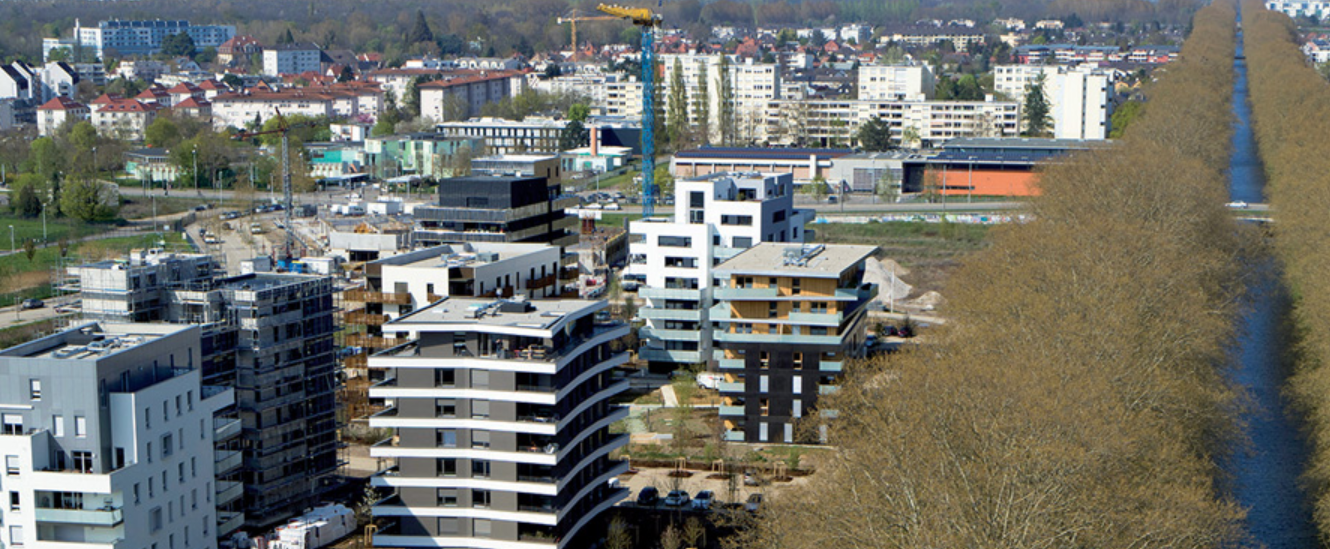
\includegraphics[width=15cm]{prairiescanal.png}
\end{center}
\caption{L'écoquartier Les Prairies du Canal en cours de construction}
\end{figure}







\chapter{Analyse des besoins}

\chapter{Synthèse des Données}

\section{Résumé des données}

\begin{table}[h]
\centering
\begin{tabularx}{\textwidth}{|X|X|X|X|}
\hline
\textbf{Appartement} & \textbf{Locataire} & \textbf{Contrat} & \textbf{Bâtiment}\\
\hline
Type d'appartement & Nom du locataire & Période & Numéro du Bâtiment \\
\hline
Nombre de locataires & Prénom du locataire & Montant du Loyer & Nombre d'appartements \\
\hline
Numéro du bâtiment & Contact du locatiare & & Quantité de déchet \\
\hline
Quantité de déchet & & & Consommation en eau et électricité \\
\hline
Consommation en eau et electricité & & & \\
\hline
\end{tabularx}
\caption{Tableau des données retenues pour la modélisation}
\end{table}

\section{Explication concernant le choix des données}

Bien qu'une grande partie de ces données répondent directements à la problématique énoncée plus tôt. Nous avons pris la liberté d'en ajouter quelques une qui permettront une meillleure gestion de cet ecoquartier, notamment :
\begin{itemize}
\item \textbf{Le nom, prénom et contact du locataire :} Dans l'optique de promouvoir chez ses locataires une gestion plus durable de leurs déchets, notre client nous a fait part de son envie d'organiser des événements les impliquant directement dans ce processus, aussi avons-nous pensé utile de permettre de trouver facilement un moyen de les joindre.
\item \textbf{La consommation et les déchets par appartement :} Notre client souhaitait avoir cette valeur pour chaque bâtiment. Cette donnée supplémentaire offrira toujours cette possibilité, en plus de pouvoir cibler des appartements plus énergivores. Il sera ainsi possible de réfléchir à une solution pour diminuer leur impact sur la consommation globale d'un bâtiment.
\end{itemize}


\chapter{Proposition de modélisation}

\section{Le MCD}

\begin{figure}[!h]
\begin{center}
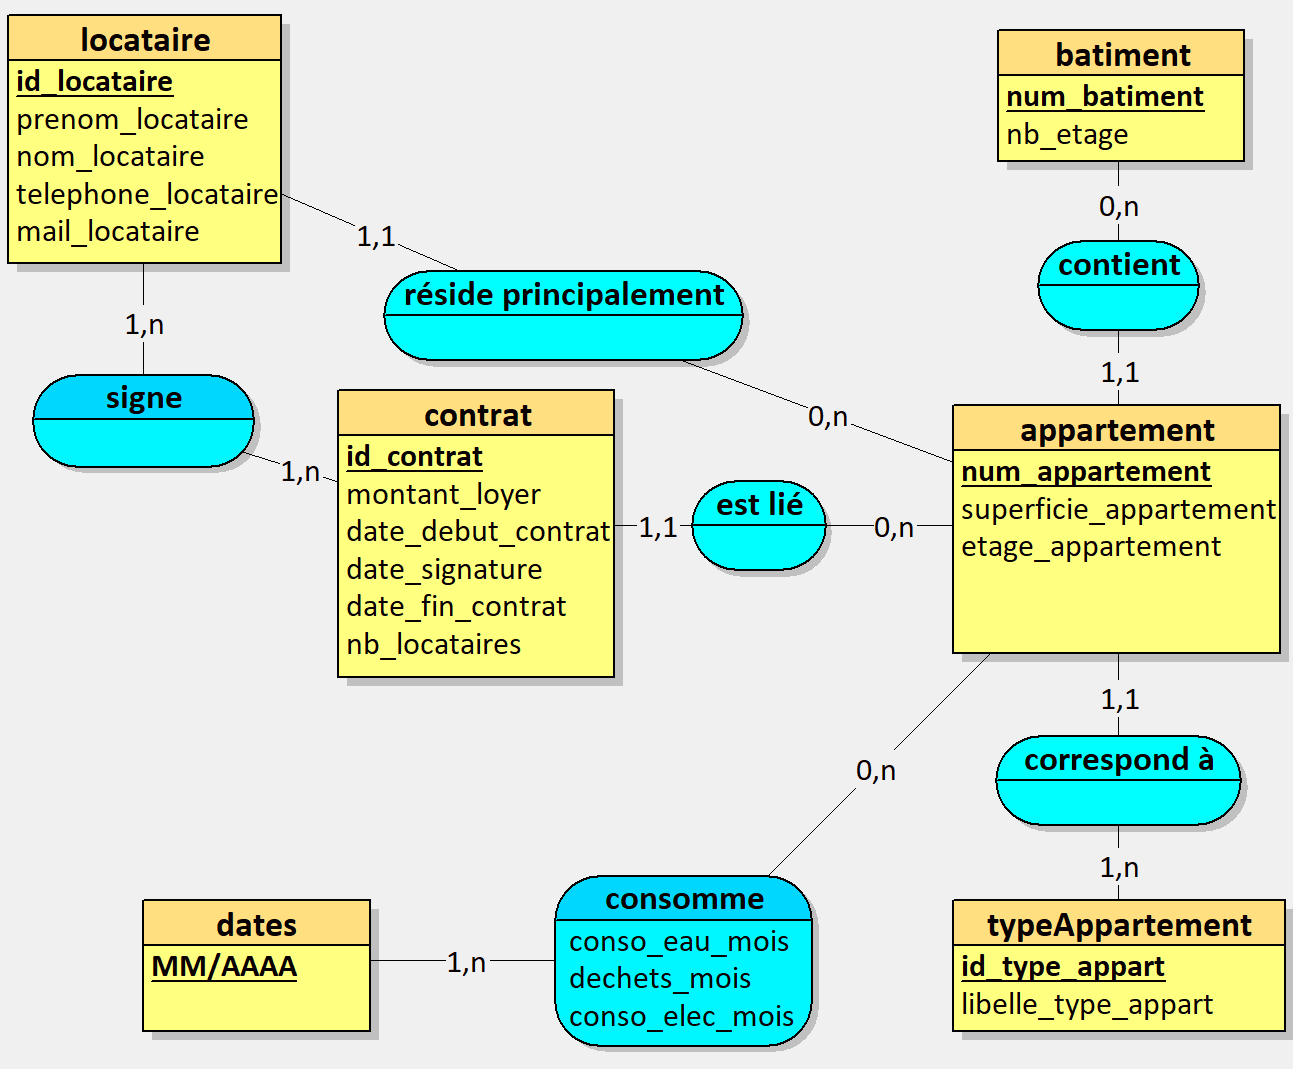
\includegraphics[width=15cm]{mcd.png}
\end{center}
\caption{Modèle conceptuel de données permettant de répondre au besoin énoncé plus tôt}
\end{figure}

\section{Explication et Justification de ce choix}

\subsection{Locataires et Contrats}

Nous avons créé l’entité locataire, qui sera identifiable par id\_locataire, cette entité contiendra le prénom, le nom, le téléphone et le mail de chaque locataire afin d’avoir leur contact complet. Un contrat est associé à un locataire par une signature, ce même contrat sera identifiable par l’identifiant id\_contrat, et contiendra le prix du loyer, la date de début du contrat, la date de signature, la date de fin du contrat et le nombre de locataires. Ces informations permettront de calculer la durée d’un contrat mais aussi de comprendre qu'une consommation puisse être plus élevé dans un appartement habité par plusieurs personnes. Par ailleurs, nous avons choisi comme cardinalité 1,n des deux côtés de l'association "signe" car un contrat doit être signé par minimum un locataire mais peut-être signé par plusieurs locataires dans le cas d'une colocation. De la même façon un contrat peut contenir 1 ou plusieurs locataire (mais jamais aucun sinon ce contrat n'a pas d'intérêt).

\subsection{Bâtiments et Appartements}

Un contrat permet à un locataire de louer un seul appartement comme l'indique la cardinalité 1,1 sortant de contrat vers appartement, en revanche, on conservera tous les contrats qui ont été liés à un appartement comme l'indique la cardinalité 0,n à droite de l'association "est lié" (on considère aussi qu’il est possible qu’un appartement qui vient d’être ajouté dans la base de données puisse ne pas avoir de contrat). L’entité appartement contient son numéro (unique pour chaque appartement permettant d'être l'identifiant de cette entité), la superficie de celui-ci, et le numéro d’étage. On notera aussi qu'un locataire peut résider principalement dans un seul et unique appartement bien qu'il puisse potentiellement avoir signé plusieurs contrat d'où la cardinalité 1,1 à gauche de l'association et 0,n à droite.\\

L’entité bâtiment sera identifiable par le numéro du bâtiment, cette entité aura une propriété nombre d’étages pour connaître le nombre d’étages du bâtiment. Il y aura une association contient entre l’entité bâtiment et l’entité appartement. En effet, l’entité bâtiment peut ne pas avoir d’appartements ou en contenir plusieurs, d’où la cardinalité de 0,n. Cependant, un appartement doit obligatoirement appartenir à un bâtiment et ne peut appartenir qu’à un seul bâtiment, nous avons donc comme cardinalité 1,1.
	 
Nous avons également une entité type d’appartement nous permettant de connaitre le nombre de pièces des appartements. Un appartement ne peut correspondre qu'a un seul type (cardinalité 1,1 vers typeAppartement) mais plusieurs appartement peuvent avoir le même type (cardinalité 1,n de typeAppartement vers appartement). On considère qu'un type n'existe pas tant qu'il n'a pas été employé pour concevoir un appartement.

\subsection{consommation}

L'association consomme entre l’entité appartement et l’entité dates porte les propriétés de consommation d'eau, d'électricité et les déchets produits. On pourra conserver un historique grâce à l'entité dates. Un appartement peut ne pas avoir de consommation d’eau, d’électricité et de déchets ou peut un ou plusieurs relevé de sa consommations qui lui sont reliés d'où une cardinalité de 0,n d'appartement vers l'association consomme.\\

Une date ne sera enregistré que si une consommation a été relevé durant cette dernière. Il va de soit qu'à une date peut correspondre plusieurs relevés provenant de différents appartements d'où le choix d'une cardinalité 1,n de consomme vers dates.


\end{document}